% !TEX root = ./robust.tex

\section{Experiments}
\label{sec:experiments}

In this section we discuss experimental results that illustrate and confirm the theoretical behavior of
median regression with corrupted data. In particular, we examine the scaling behavior of the error
with respect the level of corruption as the sample size, dimension, and correlation between predictor variables
are varied.

\subsection{Implementation}

We begin by observing that the robust lasso is equivalent to median regression for transformed data. Specifically, the robust lasso estimator can be rewritten as
\begin{align*}
  \hat\beta &= \argmin_\beta \left\{ \frac{1}{n}\|y - X\beta\|_1 + \lambda \|\beta\|_1 \right\} \\
  &= \argmin_\beta \left\{ \|y - X\beta\|_1 + \lambda n \|\beta\|_1 \right\} \\
  &= \argmin_\beta \|\tilde y - \tilde X_\lambda \beta\|_1
\end{align*}
where $\tilde y^T = (y^T, 0_p^T)$  and $\tilde X_\lambda^T = (X^T, \lambda n I_p)$.
We take $\lambda n = c\sqrt{n \log (2p)}$ for some constant $c$.

Using this reduction, we can carry out the estimation by
median regression of $\tilde y$ on $\tilde X_\lambda$. In all of our experiments below, the \texttt{quantreg} package in $R$ is used to carry out quantile regression for quantile level $\tau = \frac{1}{2}$. We do not tune the constant $c$, simply taking $c=0.5$.



\subsection{Scaling behavior with $n$ and $p$}


We first show two examples that illustrate the robustness of median regression
in the case of a single predictor variable. Here the noise $P_i$ is heteroskedastic; while Theorem~\ref{thm:main} assumes the noise is independent of the design, careful inspection of the proof suggests that the assumptions might be relaxed to allow $P_i$ to be weakly dependent, while requiring that $Q_i$ is independent of the design. 

In this simulation 75\% of the response values are corrupted. In spite of the large fraction of corrupted values, the estimated slope is very close to the true parameter. We can gain some intuition for this by observing that since the corrupting noise is independent of the predictor variable, the outliers are ``parallel'' to the regression function. 

\begin{figure*}[t]
  \begin{tabular}{cc}
    \hskip-3pt
    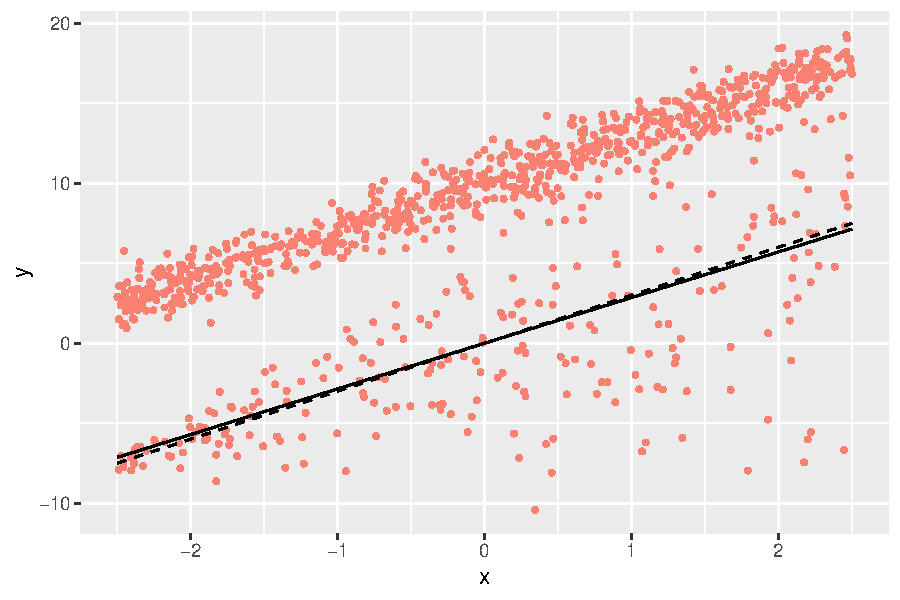
\includegraphics[width=.48\textwidth]{figures/fig1a} &
    \hskip-3pt
    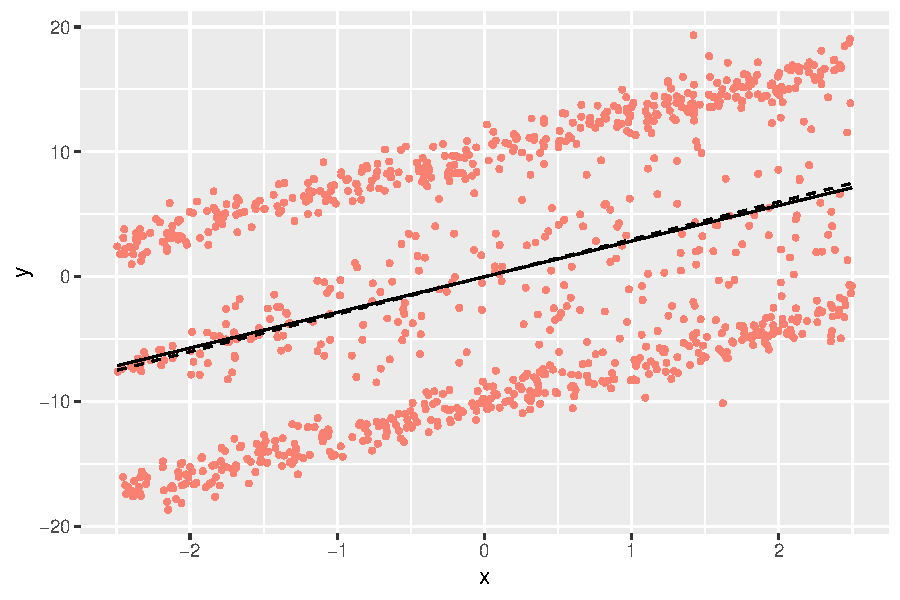
\includegraphics[width=.48\textwidth]{figures/fig1b}\\[-5pt]
  \end{tabular}
\caption{Median regression for corrupted data with $n=1{,}000$ and $\epsilon=0.75$.
The baseline noise is heteroskedastic, with distribution $P_i = N(0, (1.5 x_i + 4)^2)$
for data point $x_i$. Left: Corrupting distributions
$Q_i = N(10, 1)$. Right: Corrupting distributions $Q_i = N(10 \cdot W_i, 1)$ where $W_i$ are
independent Rademacher random variables. The solid line is the true regression
function, and the dashed line is the fit using median regression.}
\label{fig:exp}
\end{figure*}
 
In the next simulation we fix the sample size at $n=100$ and the number of non-zero coefficients $\beta^*_j$ to $s=1$. We generate $n$ data points $(X_i, y_i)$ where $y_i = X_i^T \beta^* + z_i$ with $z_i$ an additive noise term distributed
as $z_{i} \sim (1-\epsilon) N(0,1) + \epsilon\/ Q$ with $Q=N(10,1)$.

We vary the model dimension $p$ as $p_{j} = e^{\rho^j}$, rounded down to the nearest integer, for $j=0,\ldots, 10$ with $\rho=1.2$. This gives the sequence of dimensions $p=2, 3, 4, 5, 7, 12, 19, 35, 73, 174, 488$. 
Our theory implies that the squared error $\|\hat \beta - \beta^*\|^2$ of the estimator will start to rapidly increase at a critical corruption level $\epsilon^*_j$ that decreases according to
$$ \epsilon^*_{j} \approx 1- \sqrt{\rho}^j (1-\epsilon^*_0).$$
The simulation shown in Figure~\ref{fig:exp1} (left) is consistent with this theory.
Next, we fix the dimension at $p=10$ and the sparsity level at $s=5$ relevant variables. In this case
the sample size varies according to $n_j = 2^j \cdot 20$ for $j=0,\ldots, 9$. The results are
are shown in Figure~\ref{fig:exp1} (right).


\begin{figure*}[t]
\vskip20pt
  \begin{center}
    \begin{tabular}{cc}
      \hskip-10pt
      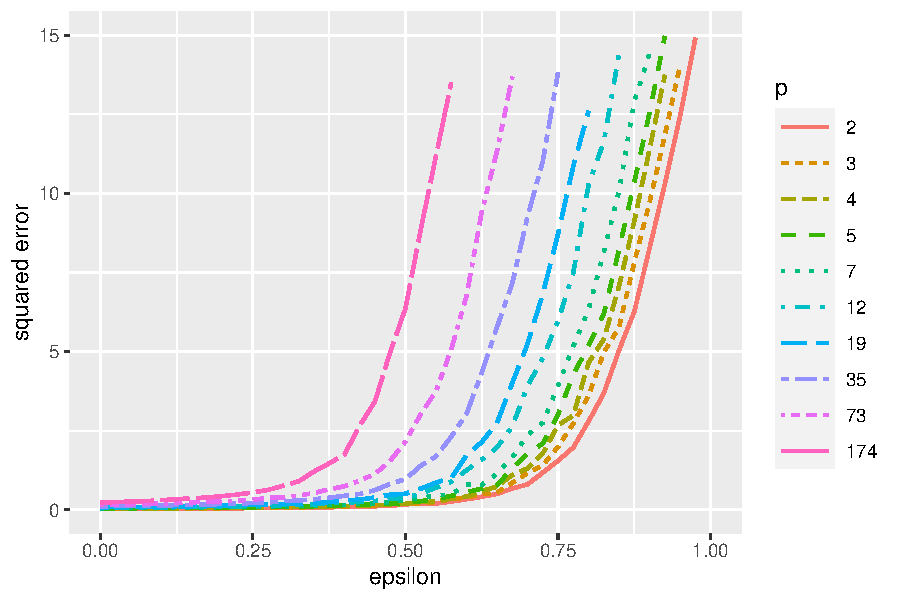
\includegraphics[width=.48\textwidth]{figures/fig2a}&
      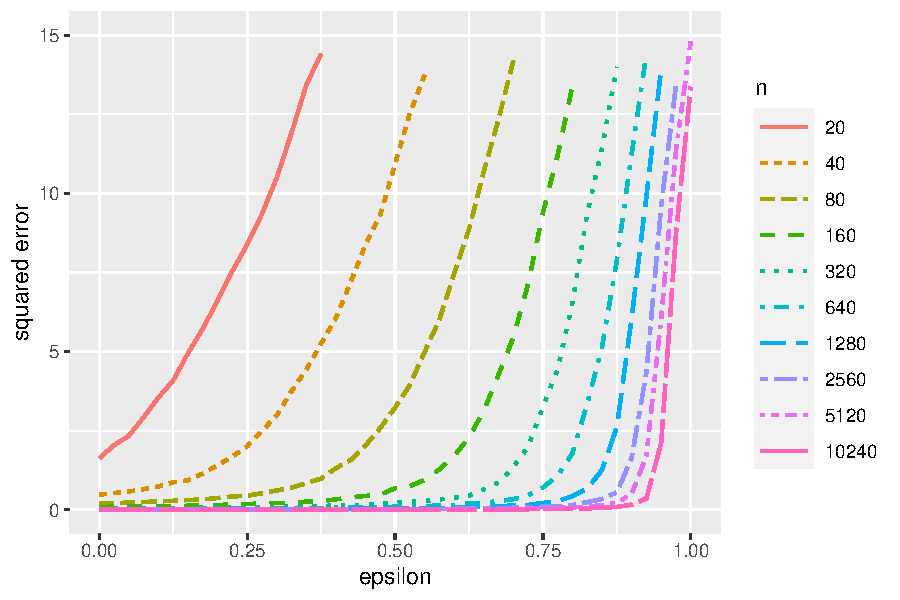
\includegraphics[width=.48\textwidth]{figures/fig2b}\\[-5pt]
    \end{tabular}
  \end{center}
\caption{Robust lasso for the linear model  $y=X\beta + z$ with design points $X_{ij}\sim N(0,1)$.
Left: Dimension $p$ varying as $p_{j} = e^{\rho^j}$, rounded down to the nearest integer, with $\rho=1.2$; the sample size is fixed at $n=100$, and $s=2$. Right: Dimension fixed at $p=10$ with $s=5$ relevant variables; the sample size $n$ is varied according to
$n_j = 2^j \cdot 20$ for $j=0,\ldots, 9$. The vertical axis shows the squared error $\|\hat \beta - \beta^*\|^2$ averaged over multiple trials.}
\label{fig:exp1}
\end{figure*}

\subsection{Correlated design}

\begin{figure*}[ht]
  \vskip20pt
    \begin{center}
      \begin{tabular}{c}
        \includegraphics[width=.50\textwidth]{figures/fig3}
      \end{tabular}
    \end{center}
  \caption{Robust lasso for the linear model  $y=X^T\beta + z$ with 
  fixed dimension $p = s$ and columns correlated pairwise with correlation 
  $2\tau/(1+\tau^2)$ varying as $\frac{3}{4} - \frac{1}{2^j}$. The sample size is fixed at $n=3000$. Each point is an average over $750$ trials.}
  \label{fig:corr}
  \end{figure*}
  
Finally, we study the effect that correlation in the design has on the robustness properties
of the estimator. This relates to 
the ratio $\overline{\kappa}/\underline{\kappa}$ characterizing the condition number of the design.
Here we fix $n=3000$, $p=10$, $s=10$, and correlate pairs of columns of $X_{i}$ and $X_{i+1}$
through a transformation 
\begin{equation*}
  (X_{i} \; X_{i+1}) = (Z_{i} \; Z_{i+1}) \begin{pmatrix}1 & \tau \\ \tau & 1\end{pmatrix}
\end{equation*}
where $Z_i$ are columns of standard normal variables; the pairwise correlations are then $2\tau/(1+\tau^2)$.
The parameter $\tau$ varies according to $\frac{3}{4} - \frac{1}{2^j}$ 
for $j=1,2,\ldots 6$. Figure~\ref{fig:corr} shows how the robustness of the estimator is reduced as the correlation increases.

